\documentclass[12pt,a4paper]{article}

% ── Packages ──
\usepackage[utf8]{inputenc}
\usepackage[T1]{fontenc}
\usepackage{lmodern}
\usepackage[margin=2.5cm]{geometry}
\usepackage{amsmath,amssymb,amsthm}
\usepackage{mathtools}
\usepackage{booktabs}
\usepackage{tabularx}
\usepackage{longtable}
\usepackage{graphicx}
\usepackage{float}
\usepackage{caption}
\usepackage{subcaption}
\usepackage[dvipsnames,svgnames,x11names]{xcolor}
\usepackage{tcolorbox}
\tcbuselibrary{skins,breakable,listings}
\usepackage{listings}
\usepackage{hyperref}
\usepackage{fancyhdr}
\usepackage{titlesec}
\usepackage{enumitem}
\usepackage{natbib}
\usepackage{algorithm}
\usepackage{algpseudocode}
\usepackage{tikz}
\usetikzlibrary{arrows.meta,positioning,shapes.geometric}

% ── Colors ──
\definecolor{primaryblue}{HTML}{2563EB}
\definecolor{deepblue}{HTML}{1E40AF}
\definecolor{accentgreen}{HTML}{059669}
\definecolor{warmamber}{HTML}{D97706}
\definecolor{lightbg}{HTML}{F0F4FF}
\definecolor{codebg}{HTML}{F8FAFC}
\definecolor{boxborder}{HTML}{BFDBFE}
\definecolor{theorembg}{HTML}{EEF2FF}
\definecolor{examplebg}{HTML}{ECFDF5}
\definecolor{warningbg}{HTML}{FEF3C7}
\definecolor{tipbg}{HTML}{F0FDF4}

% ── Hyperref ──
\hypersetup{
  colorlinks=true, linkcolor=deepblue, citecolor=accentgreen,
  urlcolor=primaryblue, bookmarks=true, bookmarksopen=true,
  pdftitle={QQKRLS: A Complete Guide},
  pdfauthor={Dr. Merwan Roudane},
}

% ── Headers ──
\pagestyle{fancy}
\fancyhf{}
\fancyhead[L]{\textcolor{primaryblue}{\small\textsc{QQKRLS Technical Guide}}}
\fancyhead[R]{\textcolor{primaryblue}{\small\thepage}}
\renewcommand{\headrulewidth}{0.5pt}
\renewcommand{\headrule}{\hbox to\headwidth{\color{primaryblue}\leaders\hrule height \headrulewidth\hfill}}

% ── Section Formatting ──
\titleformat{\section}{\Large\bfseries\color{deepblue}}{{\color{primaryblue}\thesection}}{1em}{}[\vspace{-0.5em}\textcolor{primaryblue}{\rule{\textwidth}{0.8pt}}]
\titleformat{\subsection}{\large\bfseries\color{deepblue!80!black}}{{\color{primaryblue}\thesubsection}}{0.8em}{}
\titleformat{\subsubsection}{\normalsize\bfseries\color{deepblue!60!black}}{{\color{primaryblue}\thesubsubsection}}{0.6em}{}

% ── Tcolorbox styles ──
\newtcolorbox{definitionbox}[1][]{enhanced,breakable,colback=theorembg,colframe=primaryblue,
  title={\textbf{#1}},fonttitle=\bfseries\color{white},coltitle=white,
  colbacktitle=primaryblue,boxrule=0.8pt,arc=4pt,left=8pt,right=8pt,top=6pt,bottom=6pt}

\newtcolorbox{theorembox}[1][]{enhanced,breakable,colback=theorembg,colframe=deepblue,
  title={\textbf{#1}},fonttitle=\bfseries\color{white},coltitle=white,
  colbacktitle=deepblue,boxrule=0.8pt,arc=4pt,left=8pt,right=8pt,top=6pt,bottom=6pt}

\newtcolorbox{examplebox}[1][]{enhanced,breakable,colback=examplebg,colframe=accentgreen,
  title={\textbf{#1}},fonttitle=\bfseries\color{white},coltitle=white,
  colbacktitle=accentgreen,boxrule=0.8pt,arc=4pt,left=8pt,right=8pt,top=6pt,bottom=6pt}

\newtcolorbox{warningbox}[1][]{enhanced,breakable,colback=warningbg,colframe=warmamber,
  title={\textbf{#1}},fonttitle=\bfseries\color{white},coltitle=white,
  colbacktitle=warmamber,boxrule=0.8pt,arc=4pt,left=8pt,right=8pt,top=6pt,bottom=6pt}

\newtcolorbox{tipbox}[1][]{enhanced,breakable,colback=tipbg,colframe=accentgreen!70!black,
  title={\textbf{#1}},fonttitle=\bfseries\color{white},coltitle=white,
  colbacktitle=accentgreen!70!black,boxrule=0.8pt,arc=4pt,left=8pt,right=8pt,top=6pt,bottom=6pt}

% ── Code listing style ──
\lstdefinestyle{pythonstyle}{
  language=Python, basicstyle=\small\ttfamily,
  backgroundcolor=\color{codebg}, frame=single, rulecolor=\color{boxborder},
  keywordstyle=\bfseries\color{deepblue}, stringstyle=\color{accentgreen},
  commentstyle=\itshape\color{gray}, showstringspaces=false,
  breaklines=true, numbers=left, numberstyle=\tiny\color{gray},
  xleftmargin=1.5em, framexleftmargin=1.5em, tabsize=4, captionpos=b,
}
\lstset{style=pythonstyle}

% ── Theorems ──
\newtheorem{theorem}{Theorem}[section]
\newtheorem{proposition}[theorem]{Proposition}
\newtheorem{lemma}[theorem]{Lemma}
\newtheorem{corollary}[theorem]{Corollary}
\theoremstyle{definition}
\newtheorem{definition}[theorem]{Definition}
\newtheorem{example}[theorem]{Example}
\newtheorem{remark}[theorem]{Remark}

% ── Commands ──
\newcommand{\R}{\mathbb{R}}
\newcommand{\E}{\mathbb{E}}
\newcommand{\Var}{\operatorname{Var}}
\newcommand{\Hk}{\mathcal{H}_K}
\newcommand{\bx}{\mathbf{x}}
\newcommand{\by}{\mathbf{y}}
\newcommand{\bc}{\mathbf{c}}
\newcommand{\bK}{\mathbf{K}}
\newcommand{\bI}{\mathbf{I}}
\newcommand{\bV}{\mathbf{V}}
\newcommand{\bLambda}{\boldsymbol{\Lambda}}

\begin{document}

% ── TITLE PAGE ──
\begin{titlepage}
\begin{center}
\vspace*{2cm}
{\Huge\bfseries\textcolor{deepblue}{QQKRLS}}\\[0.5cm]
{\LARGE\textcolor{primaryblue}{Quantile-on-Quantile Kernel-Based\\[0.2cm] Regularized Least Squares}}\\[1.5cm]
{\Large\textcolor{deepblue!70!black}{A Complete Technical Guide}}\\[0.3cm]
{\large\textcolor{gray}{From Zero to Expert --- For Researchers \& Practitioners}}\\[3cm]

\textcolor{primaryblue}{\rule{0.6\textwidth}{1.5pt}}\\[1cm]

{\Large \textbf{Dr.\ Merwan Roudane}}\\[0.4cm]
{\normalsize \texttt{merwanroudane920@gmail.com}}\\[0.3cm]
{\small
\textcolor{primaryblue}{\textbf{PyPI:}} \url{https://pypi.org/project/qqkrls/}\\
\textcolor{accentgreen}{\textbf{GitHub:}} \url{https://github.com/merwanroudane/qqkrls}
}\\[2cm]

{\large Version 1.1.1}\\[0.5cm]
{\normalsize \today}
\end{center}
\end{titlepage}

\tableofcontents
\newpage

% ── Include all parts ──
% ═══════════════════════════════════════════════════════════════════
%  PART 1: Introduction & KRLS Theory
% ═══════════════════════════════════════════════════════════════════

\section{Introduction}

\begin{tipbox}[Who Is This Guide For?]
This guide is written for \textbf{researchers, graduate students, and practitioners} in economics, finance, and environmental science who want to apply advanced nonparametric methods without requiring deep machine-learning expertise. We start from basic regression concepts and build up to the full QQKRLS estimator.
\end{tipbox}

\subsection{Motivation: Why Go Beyond OLS?}

Ordinary Least Squares (OLS) is the workhorse of empirical economics. Given a model $y = X\beta + \varepsilon$, OLS provides the best linear unbiased estimator (BLUE) under the Gauss--Markov assumptions. However, OLS imposes strong restrictions:

\begin{enumerate}[label=\textcolor{primaryblue}{\arabic*.}]
\item \textbf{Linearity}: The conditional expectation $\E[y \mid x]$ must be linear in $x$.
\item \textbf{Additivity}: Each predictor's effect is separable --- no automatic interactions.
\item \textbf{Homogeneity}: The effect $\beta_j$ is \emph{constant} across the entire distribution.
\end{enumerate}

In reality, economic relationships are often \textbf{nonlinear}, \textbf{interactive}, and \textbf{heterogeneous across the distribution}. For example, the effect of energy consumption on environmental quality may differ at low vs.\ high consumption levels.

\begin{warningbox}[The Problem with Misspecification]
If the true data-generating process is nonlinear but we fit a linear model, OLS estimates are \textbf{biased and inconsistent}. Diagnostic tests (Ramsey RESET, BDS) can detect this misspecification, but the solution requires a more flexible estimator.
\end{warningbox}

\subsection{The QQKRLS Framework}

The \texttt{qqkrls} library provides a unified solution through four methods:

\begin{center}
\begin{tabular}{>{\bfseries\color{deepblue}}l p{10cm}}
\toprule
\textbf{Method} & \textbf{Description} \\
\midrule
KRLS & Kernel Regularized Least Squares --- nonparametric regression in a reproducing kernel Hilbert space \\
QQ Regression & Quantile-on-Quantile analysis --- examines how effects vary across both distributions \\
WQR & Weighted Quantile Regression --- kernel-weighted quantile estimates \\
QQKRLS & The combined estimator --- nonparametric marginal effects across all quantile pairs \\
\bottomrule
\end{tabular}
\end{center}


% ═══════════════════════════════════════════════════════════════════
\section{Kernel Regularized Least Squares (KRLS)}
% ═══════════════════════════════════════════════════════════════════

\subsection{Intuition: From Linear to Nonparametric}

Consider the classical regression problem: given data $\{(x_i, y_i)\}_{i=1}^N$ where $x_i \in \R^D$ and $y_i \in \R$, we want to estimate the conditional expectation function $f(x) = \E[y \mid x]$.

\begin{itemize}[leftmargin=2em]
\item \textbf{OLS}: Restricts $f(x) = x^\top \beta$ --- a linear function.
\item \textbf{KRLS}: Allows $f$ to be \emph{any smooth function} in a reproducing kernel Hilbert space $\Hk$.
\end{itemize}

The key insight is the \textbf{kernel trick}: instead of explicitly specifying a functional form, KRLS defines similarity between observations using a \emph{kernel function} and learns a flexible, data-driven relationship.

\subsection{The Gaussian Kernel}

\begin{definitionbox}[Definition: Gaussian (RBF) Kernel]
The Gaussian kernel measures the similarity between two observations $x_i$ and $x_j$:
\begin{equation}
K(x_i, x_j) = \exp\!\left(-\frac{\|x_i - x_j\|^2}{\sigma}\right)
\label{eq:kernel}
\end{equation}
where $\sigma > 0$ is the \textbf{bandwidth} parameter controlling the smoothness of the function.
\end{definitionbox}

\textbf{Properties:}
\begin{itemize}[leftmargin=2em]
\item $K(x_i, x_i) = 1$ --- each observation is perfectly similar to itself.
\item $K(x_i, x_j) \to 0$ as $\|x_i - x_j\| \to \infty$ --- distant observations have negligible influence.
\item \textbf{Large $\sigma$}: Broader influence $\to$ smoother function (closer to linear).
\item \textbf{Small $\sigma$}: Narrower influence $\to$ more flexible (risk of overfitting).
\end{itemize}

\begin{tipbox}[Default Bandwidth]
Following Hainmueller \& Hazlett (2014), KRLS sets $\sigma = D$ (the number of predictors). This heuristic works well in practice and avoids expensive bandwidth search.
\end{tipbox}

\subsection{The KRLS Optimization Problem}

\begin{theorembox}[KRLS Objective Function]
KRLS solves the following Tikhonov-regularized optimization:
\begin{equation}
\hat{f} = \arg\min_{f \in \Hk} \underbrace{\sum_{i=1}^{N} (y_i - f(x_i))^2}_{\text{Data fidelity}} + \underbrace{\lambda \|f\|_{\Hk}^2}_{\text{Regularization}}
\label{eq:krls_obj}
\end{equation}
where $\lambda > 0$ controls the trade-off between fitting the data and keeping the function smooth.
\end{theorembox}

\textbf{Interpretation:}
\begin{itemize}[leftmargin=2em]
\item The first term minimizes the sum of squared residuals (like OLS).
\item The second term penalizes complexity in the RKHS norm, preventing overfitting.
\item $\lambda \to 0$: Interpolates the data (overfitting).
\item $\lambda \to \infty$: Converges to the sample mean (underfitting).
\end{itemize}

\subsection{The Representer Theorem and Closed-Form Solution}

\begin{theorembox}[Representer Theorem (Scholkopf \& Smola, 2002)]
The minimizer of Eq.~\eqref{eq:krls_obj} has the finite representation:
\begin{equation}
\hat{f}(x) = \sum_{i=1}^{N} c_i \cdot K(x, x_i)
\label{eq:representer}
\end{equation}
where $\bc = (c_1, \ldots, c_N)^\top$ is a vector of $N$ coefficients.
\end{theorembox}

This is remarkable: although the RKHS is infinite-dimensional, the optimal solution only depends on $N$ parameters. The predicted value at any point $x$ is a \textbf{weighted sum of kernel similarities} to all training observations.

\subsubsection{Eigendecomposition Solution}

Substituting Eq.~\eqref{eq:representer} into Eq.~\eqref{eq:krls_obj} and taking the first-order condition:
\begin{equation}
\bc^* = (\bK + \lambda \bI)^{-1} \by
\label{eq:coef_basic}
\end{equation}
where $\bK$ is the $N \times N$ kernel matrix with $K_{ij} = K(x_i, x_j)$.

For numerical stability, KRLS uses the eigendecomposition $\bK = \bV \bLambda \bV^\top$:
\begin{equation}
\boxed{\bc^* = \bV (\bLambda + \lambda \bI)^{-1} \bV^\top \by}
\label{eq:coef_eigen}
\end{equation}

\begin{examplebox}[Computational Advantage]
The eigendecomposition is computed \textbf{once} and reused for different values of $\lambda$, making leave-one-out cross-validation extremely efficient.
\end{examplebox}

\subsection{Regularization Parameter Selection via LOO-CV}

\begin{definitionbox}[Leave-One-Out Cross-Validation]
The LOO-CV error is:
\begin{equation}
\text{LOO}(\lambda) = \sum_{i=1}^{N} \left(\frac{y_i - \hat{f}_\lambda(x_i)}{1 - H_{ii}(\lambda)}\right)^2
\end{equation}
where $H_{ii}(\lambda)$ is the $i$-th diagonal of the hat matrix $\bH = \bK(\bK + \lambda \bI)^{-1}$.
\end{definitionbox}

KRLS selects $\lambda^*$ by minimizing this LOO error, which can be computed \textbf{without actually refitting} the model $N$ times (using the eigendecomposition).

\subsection{Pointwise Marginal Effects}

Unlike OLS (which gives one constant coefficient per variable), KRLS provides a \textbf{marginal effect for each observation}. This is computed analytically:

\begin{theorembox}[KRLS Pointwise Marginal Effect]
The marginal effect of predictor $d$ at observation $j$ is:
\begin{equation}
\frac{\partial \hat{f}(x_j)}{\partial x_j^{(d)}} = \frac{-2}{\sigma} \sum_{i=1}^{N} c_i \cdot K(x_j, x_i) \cdot \left(x_i^{(d)} - x_j^{(d)}\right)
\label{eq:deriv}
\end{equation}
\end{theorembox}

\textbf{Key insight}: The marginal effect varies by observation. If these pointwise effects show substantial variation (different at Q25 vs.\ Q75), the relationship is genuinely nonlinear, justifying KRLS over OLS.

\begin{examplebox}[Interpreting Marginal Effects]
\begin{itemize}[leftmargin=1.5em]
\item \textbf{Average Marginal Effect}: $\overline{\text{ME}}_d = \frac{1}{N}\sum_{j=1}^{N} \frac{\partial \hat{f}}{\partial x_j^{(d)}}$ --- comparable to OLS $\hat{\beta}_d$.
\item \textbf{Heterogeneity}: If Q25 $\neq$ Q75 of the effects, the relationship is nonlinear.
\item \textbf{Plots}: Scatter plots of marginal effects vs.\ predictor values reveal the functional form.
\end{itemize}
\end{examplebox}

% ═══════════════════════════════════════════════════════════════════
%  PART 2: QQ Regression & QQKRLS Theory
% ═══════════════════════════════════════════════════════════════════

\section{Quantile-on-Quantile (QQ) Regression}

\subsection{Motivation: Beyond the Mean}

Standard regression estimates the \textbf{conditional mean} $\E[y \mid x]$. But economic relationships often differ across the distribution:

\begin{itemize}[leftmargin=2em]
\item Does energy consumption affect environmental quality \emph{differently} when the footprint is already high vs.\ low?
\item Is the GDP--pollution nexus stronger during economic booms (high GDP quantiles) or recessions (low GDP quantiles)?
\end{itemize}

\textbf{Quantile regression} (Koenker, 2005) addresses the first question by estimating conditional quantiles $Q_\tau(y \mid x)$ for different $\tau \in (0,1)$. But it still assumes a \emph{fixed} effect of $x$ regardless of where $x$ falls in its own distribution.

\begin{definitionbox}[Quantile-on-Quantile Regression (Sim \& Zhou, 2015)]
QQ regression creates a \textbf{two-dimensional mapping} $\beta(\theta, \tau)$ that captures how the $\theta$-th quantile of $X$ affects the $\tau$-th conditional quantile of $Y$. This reveals distributional heterogeneity in \emph{both} variables simultaneously.
\end{definitionbox}

\subsection{The QQ Regression Procedure}

\begin{algorithm}[H]
\caption{Quantile-on-Quantile Regression}
\begin{algorithmic}[1]
\Require Data $\{(x_i, y_i)\}_{i=1}^N$, quantile grids $\Theta = \{\theta_1, \ldots, \theta_J\}$ and $\mathcal{T} = \{\tau_1, \ldots, \tau_K\}$
\Ensure Coefficient matrix $\beta(\theta, \tau)$ of dimension $K \times J$
\For{each $\theta \in \Theta$}
    \State Compute threshold: $q_\theta = Q_X(\theta)$ \Comment{$\theta$-th quantile of $X$}
    \State Subset: $\mathcal{S}_\theta = \{(x_i, y_i) : x_i \leq q_\theta\}$
    \For{each $\tau \in \mathcal{T}$}
        \State Estimate $\tau$-th quantile regression of $Y$ on $X$ using $\mathcal{S}_\theta$
        \State Store $\hat{\beta}(\theta, \tau)$
    \EndFor
\EndFor
\State \Return Matrix $[\hat{\beta}(\theta_j, \tau_k)]_{k,j}$
\end{algorithmic}
\end{algorithm}

\subsection{Interpreting the QQ Coefficient Matrix}

The result is a $K \times J$ matrix where:
\begin{itemize}[leftmargin=2em]
\item \textbf{Rows} ($\tau$): Quantiles of $Y$ (the dependent variable)
\item \textbf{Columns} ($\theta$): Quantiles of $X$ (the independent variable)
\item \textbf{Cell $\beta(\theta, \tau)$}: The marginal effect of $X$ on $Y$ at that specific distributional location
\end{itemize}

\begin{center}
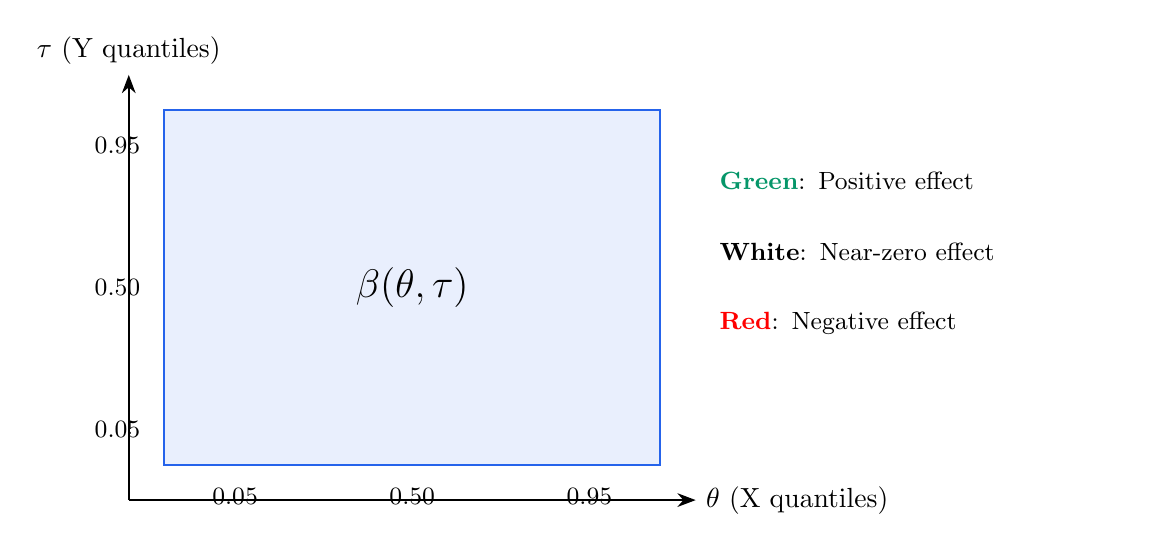
\begin{tikzpicture}[scale=0.9]
  \draw[thick,-{Stealth}] (0,0) -- (8,0) node[right] {$\theta$ (X quantiles)};
  \draw[thick,-{Stealth}] (0,0) -- (0,6) node[above] {$\tau$ (Y quantiles)};
  \fill[primaryblue!10] (0.5,0.5) rectangle (7.5,5.5);
  \draw[primaryblue,thick] (0.5,0.5) rectangle (7.5,5.5);
  \node at (4,3) {\Large $\beta(\theta, \tau)$};
  \node[below] at (1.5,0.3) {\small 0.05};
  \node[below] at (4,0.3) {\small 0.50};
  \node[below] at (6.5,0.3) {\small 0.95};
  \node[left] at (0.3,1) {\small 0.05};
  \node[left] at (0.3,3) {\small 0.50};
  \node[left] at (0.3,5) {\small 0.95};
  \node[right,text width=5cm,font=\small] at (8.2,4.5) {\textcolor{accentgreen}{\textbf{Green}}: Positive effect};
  \node[right,text width=5cm,font=\small] at (8.2,3.5) {\textbf{White}: Near-zero effect};
  \node[right,text width=5cm,font=\small] at (8.2,2.5) {\textcolor{red}{\textbf{Red}}: Negative effect};
\end{tikzpicture}
\end{center}

% ═══════════════════════════════════════════════════════════════════
\section{The QQKRLS Estimator}
% ═══════════════════════════════════════════════════════════════════

\subsection{Combining KRLS with QQ Regression}

QQKRLS (Adebayo et al., 2024) replaces the linear quantile regression step in QQ with \textbf{KRLS}, creating a fully nonparametric estimator:

\begin{theorembox}[The QQKRLS Algorithm]
For each X-quantile $\theta$ and Y-quantile $\tau$:
\begin{enumerate}[label=\textcolor{white}{\arabic*.}]
\item \textbf{Subset}: Select observations where $x_i \leq Q_X(\theta)$
\item \textbf{Fit KRLS}: Apply kernel regression on the subset $\to$ obtain pointwise marginal effects $\left\{\frac{\partial \hat{f}_{[\theta]}}{\partial x}\right\}$
\item \textbf{Extract quantile}: The coefficient is the $\tau$-th quantile of the marginal effects:
\begin{equation}
\boxed{\beta(\theta, \tau) = Q_\tau\!\left(\left\{\frac{\partial \hat{f}_{[\theta]}(x_j)}{\partial x}\right\}_{j \in \mathcal{S}_\theta}\right)}
\end{equation}
\end{enumerate}
\end{theorembox}

\subsection{Detailed QQKRLS Algorithm}

\begin{algorithm}[H]
\caption{QQKRLS Estimation with Bootstrap Inference}
\begin{algorithmic}[1]
\Require $\by, \bx$, quantile grids $\Theta, \mathcal{T}$, bootstrap replications $B$, min.\ obs.\ $n_{\min}$
\Ensure $\hat{\beta}(\theta,\tau)$, $\text{SE}(\theta,\tau)$, $t(\theta,\tau)$, $p(\theta,\tau)$
\For{each $\theta \in \Theta$}
    \State $q_\theta \gets Q_X(\theta)$; \quad $\mathcal{S}_\theta \gets \{i : x_i \leq q_\theta\}$
    \If{$|\mathcal{S}_\theta| \geq n_{\min}$}
        \State Fit KRLS on $(x_{\mathcal{S}_\theta}, y_{\mathcal{S}_\theta})$ with derivative=True
        \State Extract pointwise marginal effects $\{d_j\}_{j \in \mathcal{S}_\theta}$
        \For{each $\tau \in \mathcal{T}$}
            \State $\hat{\beta}(\theta,\tau) \gets Q_\tau(\{d_j\})$ \Comment{$\tau$-th quantile of effects}
            \For{$b = 1, \ldots, B$} \Comment{Bootstrap for SE}
                \State Draw bootstrap sample with replacement from $\mathcal{S}_\theta$
                \State Fit KRLS on bootstrap sample
                \State $\hat{\beta}^{(b)}(\theta,\tau) \gets Q_\tau$ of bootstrap marginal effects
            \EndFor
            \State $\widehat{\text{SE}} \gets \text{std}(\hat{\beta}^{(1)}, \ldots, \hat{\beta}^{(B)})$
            \State $t \gets \hat{\beta} / \widehat{\text{SE}}$; \quad $p \gets 2\Phi(-|t|)$
        \EndFor
    \EndIf
\EndFor
\end{algorithmic}
\end{algorithm}

\subsection{Why QQKRLS Improves Over Standard QQ}

\begin{center}
\begin{tabular}{>{\bfseries\color{deepblue}}l p{5.5cm} p{5.5cm}}
\toprule
& \textbf{Standard QQ} & \textbf{QQKRLS} \\
\midrule
Inner estimator & Linear quantile regression & KRLS (nonparametric) \\
Functional form & Assumes linearity within subsets & No functional form assumption \\
Interactions & Not captured & Automatic via Gaussian kernel \\
Marginal effects & Constant within each subset & Pointwise (varies by obs.) \\
Inference & Asymptotic & Bootstrap (finite-sample valid) \\
\bottomrule
\end{tabular}
\end{center}

\subsection{Statistical Inference}

\subsubsection{Bootstrap Standard Errors}

For each cell $(\theta, \tau)$, QQKRLS uses the \textbf{paired bootstrap}:
\begin{enumerate}[leftmargin=2em]
\item Draw $B$ bootstrap samples (with replacement) from the subset $\mathcal{S}_\theta$
\item Re-estimate KRLS and extract the $\tau$-th quantile of marginal effects
\item The bootstrap standard error: $\widehat{\text{SE}}(\theta,\tau) = \text{std}\{\hat{\beta}^{(1)}, \ldots, \hat{\beta}^{(B)}\}$
\end{enumerate}

\subsubsection{Test Statistics and P-values}

Under the null $H_0: \beta(\theta,\tau) = 0$:
\begin{equation}
t(\theta,\tau) = \frac{\hat{\beta}(\theta,\tau)}{\widehat{\text{SE}}(\theta,\tau)} \xrightarrow{d} \mathcal{N}(0,1)
\end{equation}
\begin{equation}
p(\theta,\tau) = 2\Phi\!\left(-|t(\theta,\tau)|\right)
\end{equation}

\begin{tipbox}[Significance Conventions]
\begin{itemize}[leftmargin=1.5em]
\item $^{***}$: $p < 0.01$ (highly significant)
\item $^{**}$: $p < 0.05$ (significant at 5\%)
\item $^{*}$: $p < 0.10$ (marginally significant)
\end{itemize}
These stars are displayed on the heatmap to show which cells have statistically significant effects.
\end{tipbox}

% ═══════════════════════════════════════════════════════════════════
%  PART 3: Diagnostics, Python Usage & Interpretation
% ═══════════════════════════════════════════════════════════════════

\section{Pre-Estimation Diagnostic Tests}

Before applying KRLS/QQKRLS, researchers must \textbf{justify} the use of nonparametric methods. The \texttt{qqkrls} library includes a complete diagnostic battery.

\subsection{Ramsey RESET Test}

\begin{definitionbox}[Ramsey RESET (Regression Equation Specification Error Test)]
Tests whether the linear model is correctly specified by including powers of fitted values:
\begin{equation}
y = X\beta + \gamma_2 \hat{y}^2 + \gamma_3 \hat{y}^3 + \varepsilon
\end{equation}
\begin{itemize}[leftmargin=1.5em]
\item $H_0$: Linear model is correctly specified ($\gamma_2 = \gamma_3 = 0$)
\item $H_1$: Nonlinear terms are significant $\to$ \textbf{use KRLS}
\end{itemize}
\end{definitionbox}

\subsection{Breusch--Pagan Test}

\begin{definitionbox}[Breusch--Pagan Test for Heteroskedasticity]
Tests whether the variance of residuals depends on the predictors:
\begin{equation}
\hat{\varepsilon}^2 = X\alpha + u
\end{equation}
\begin{itemize}[leftmargin=1.5em]
\item $H_0$: Homoskedasticity ($\Var[\varepsilon \mid X] = \sigma^2$)
\item $H_1$: Heteroskedasticity $\to$ \textbf{effects differ across distribution} $\to$ use quantile-based analysis
\end{itemize}
\end{definitionbox}

\subsection{BDS Test}

\begin{definitionbox}[BDS Test (Brock, Dechert, Scheinkman)]
A nonparametric test for serial independence and nonlinear structure in the residuals:
\begin{itemize}[leftmargin=1.5em]
\item $H_0$: Residuals are i.i.d.
\item $H_1$: Nonlinear dependence exists $\to$ \textbf{justifies KRLS/QQKRLS}
\end{itemize}
The test uses the correlation integral at embedding dimension $m$:
\begin{equation}
C_m(\epsilon) = \lim_{N \to \infty} \frac{2}{N(N-1)} \sum_{i<j} \mathbf{1}\!\left[\|x_i^m - x_j^m\| < \epsilon\right]
\end{equation}
Under the null, $C_m(\epsilon) = [C_1(\epsilon)]^m$. The BDS statistic tests this equality.
\end{definitionbox}

\subsection{Jarque--Bera Normality Test}

\begin{definitionbox}[Jarque--Bera Test]
Tests whether the data follows a normal distribution:
\begin{equation}
JB = \frac{N}{6}\left(S^2 + \frac{(K-3)^2}{4}\right) \sim \chi^2(2)
\end{equation}
where $S$ = skewness, $K$ = kurtosis. Rejection suggests \textbf{non-Gaussian distributions}, motivating quantile-based methods.
\end{definitionbox}

\subsection{Andrews Parameter Stability Test}

\begin{definitionbox}[Andrews Sup-F Test]
Tests for structural breaks in the relationship by computing $F$-statistics at all possible break points:
\begin{itemize}[leftmargin=1.5em]
\item \textbf{Max-F}: Supreme of $F$-statistics (detects single break)
\item \textbf{Exp-F}: Exponential average (robust to multiple breaks)
\item \textbf{Ave-F}: Simple average (overall instability)
\end{itemize}
Parameter instability justifies quantile-based methods that allow coefficients to vary.
\end{definitionbox}


\section{Using the \texttt{qqkrls} Python Library}

\subsection{Installation}

\begin{lstlisting}[language=bash,style=pythonstyle]
pip install qqkrls
\end{lstlisting}

\subsection{Complete Workflow}

\begin{lstlisting}
import numpy as np
import pandas as pd
from qqkrls import (
    krls, qqkrls, predict_krls,
    plot_qqkrls_heatmap, plot_qqkrls_3d,
    plot_qqkrls_contour, plot_qqkrls_pvalue,
    plot_krls_derivatives, plot_krls_fit,
    descriptive_statistics, linearity_test_battery,
    bds_test, jarque_bera, print_diagnostics,
)

# Step 1: Load data
y = df['EF'].values
X = df[['Energy', 'CO2', 'GDP']].values

# Step 2: Pre-estimation diagnostics
diag = linearity_test_battery(y, X, col_names=['Energy','CO2','GDP'])
print_diagnostics(diag)

# Step 3: Fit KRLS
fit = krls(X, y, derivative=True, vcov=True, verbose=1)

# Step 4: QQKRLS estimation
taus = np.arange(0.05, 1.0, 0.05)
result = qqkrls(y=y, x=df['Energy'].values,
                y_quantiles=taus, x_quantiles=taus,
                n_boot=200, verbose=True)

# Step 5: Visualize
plot_qqkrls_heatmap(result, colorscale='paper',
                    show_stars=True, save_path='heatmap.png')
plot_qqkrls_3d(result, save_path='surface.png')
\end{lstlisting}

\subsection{Key API Functions}

\begin{center}
\small
\begin{tabular}{>{\ttfamily\color{deepblue}}l p{8cm}}
\toprule
\textbf{Function} & \textbf{Description} \\
\midrule
krls(X, y) & Fit KRLS model with LOO cross-validation \\
qqkrls(y, x) & Run QQKRLS with bootstrap inference \\
predict\_krls(fit, X\_new) & Out-of-sample prediction \\
\midrule
plot\_qqkrls\_heatmap() & Paper-style coefficient heatmap \\
plot\_qqkrls\_3d() & MATLAB-style 3D surface plot \\
plot\_qqkrls\_contour() & Filled contour plot \\
plot\_qqkrls\_pvalue() & P-value significance map \\
plot\_qqkrls\_panel() & Multi-variable panel \\
plot\_krls\_derivatives() & Marginal effect scatter + density \\
plot\_krls\_fit() & Fitted vs actual with $R^2$ \\
\midrule
descriptive\_statistics() & LaTeX descriptive statistics table \\
qqkrls\_coefficient\_table() & LaTeX coefficient matrix \\
krls\_summary\_table() & LaTeX KRLS summary \\
export\_results\_csv() & CSV export of all results \\
\midrule
linearity\_test\_battery() & RESET + BP + JB + BDS \\
bds\_test() & BDS independence test \\
parameter\_stability\_test() & Andrews sup-F, exp-F, ave-F \\
jarque\_bera() & Jarque--Bera normality test \\
\bottomrule
\end{tabular}
\end{center}


\section{Interpreting QQKRLS Results}

\subsection{Reading the Heatmap}

The QQKRLS heatmap is the primary output. Each cell $(\theta, \tau)$ represents one nonparametric marginal effect:

\begin{warningbox}[Common Misinterpretations to Avoid]
\begin{itemize}[leftmargin=1.5em]
\item The axes are \textbf{quantiles}, not raw values of the variables.
\item $\theta = 0.05$ means ``when $X$ is at its 5th percentile,'' not ``when $X = 0.05$.''
\item A positive coefficient means: at that distributional location, increasing $X$ \emph{increases} $Y$.
\end{itemize}
\end{warningbox}

\subsection{Pattern Recognition}

\begin{center}
\begin{tabular}{>{\bfseries\color{deepblue}}l p{9cm}}
\toprule
\textbf{Pattern} & \textbf{Economic Interpretation} \\
\midrule
Uniform positive & $X$ always increases $Y$ (homogeneous positive effect) \\
Gradient left-to-right & Effect strengthens as $X$ increases (nonlinear amplification) \\
Gradient bottom-to-top & Effect stronger when $Y$ is high (asymmetric vulnerability) \\
Diagonal pattern & Effect strongest at matching quantiles (distributional symmetry) \\
Quadrant split & Effect changes sign across the distribution (regime switching) \\
Significance clusters & Only certain quantile pairs show significant effects \\
\bottomrule
\end{tabular}
\end{center}

\subsection{Writing Up Results for a Paper}

\begin{examplebox}[Template for Results Section]
``Table X presents the QQKRLS estimates of the marginal effect of [Variable] on [Dependent Variable] across 19 quantile pairs ($\theta, \tau \in \{0.05, 0.10, \ldots, 0.95\}$). The pre-estimation diagnostics (Ramsey RESET: $F = \ldots$, $p = \ldots$; BDS: $z = \ldots$, $p < 0.01$) reject linearity and i.i.d.\ residuals, justifying the nonparametric QQKRLS approach.

The heatmap in Figure Y reveals substantial heterogeneity across the distribution. At lower quantiles of [Variable] ($\theta < 0.30$), the effect on [DV] is [negative/insignificant], while at upper quantiles ($\theta > 0.70$), the effect becomes [significantly positive]. This asymmetry suggests that [economic interpretation].

Of the 361 quantile-pair cells, [N] ([\%]\%) are significant at the 5\% level, concentrated in the [describe region] of the heatmap. These findings are robust to the bootstrap inference with $B = 200$ replications.''
\end{examplebox}

\subsection{Methodological Justification Workflow}

The recommended workflow for any QQKRLS paper follows five steps:

\begin{center}
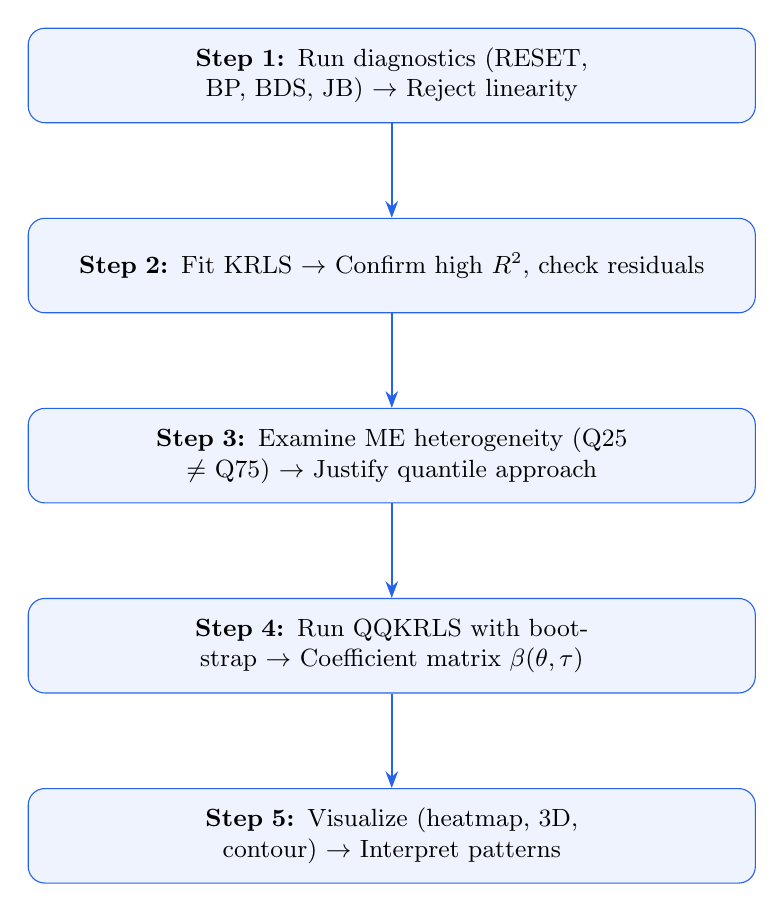
\begin{tikzpicture}[
  node distance=1.2cm,
  box/.style={rectangle, rounded corners=6pt, draw=primaryblue, fill=primaryblue!8, text width=9cm, minimum height=1.2cm, align=center, font=\small},
  arrow/.style={-{Stealth[length=6pt]}, thick, primaryblue}
]
\node[box] (s1) {\textbf{Step 1:} Run diagnostics (RESET, BP, BDS, JB) $\to$ Reject linearity};
\node[box, below=of s1] (s2) {\textbf{Step 2:} Fit KRLS $\to$ Confirm high $R^2$, check residuals};
\node[box, below=of s2] (s3) {\textbf{Step 3:} Examine ME heterogeneity (Q25 $\neq$ Q75) $\to$ Justify quantile approach};
\node[box, below=of s3] (s4) {\textbf{Step 4:} Run QQKRLS with bootstrap $\to$ Coefficient matrix $\beta(\theta, \tau)$};
\node[box, below=of s4] (s5) {\textbf{Step 5:} Visualize (heatmap, 3D, contour) $\to$ Interpret patterns};
\draw[arrow] (s1) -- (s2);
\draw[arrow] (s2) -- (s3);
\draw[arrow] (s3) -- (s4);
\draw[arrow] (s4) -- (s5);
\end{tikzpicture}
\end{center}


% ── Bibliography ──
\newpage
\section{References}

\begin{enumerate}[leftmargin=2em]
\item \textbf{Hainmueller, J.\ \& Hazlett, C.} (2014). Kernel Regularized Least Squares: Moving Beyond Linearity and Additivity without Sacrificing Interpretability. \textit{Political Analysis}, 22(2), 143--168. \href{https://doi.org/10.1093/pan/mpt024}{doi:10.1093/pan/mpt024}

\item \textbf{Sim, N.\ \& Zhou, H.} (2015). Oil Prices, US Stock Return, and the Dependence Between Their Quantiles. \textit{Journal of Banking \& Finance}, 55, 1--12. \href{https://doi.org/10.1016/j.jbankfin.2015.01.013}{doi:10.1016/j.jbankfin.2015.01.013}

\item \textbf{Adebayo, T.S., Ozkan, O.\ \& Eweade, B.S.} (2024). Do energy efficiency R\&D investments and ICT promote environmental sustainability in Sweden? A novel QQKRLS investigation. \textit{Journal of Cleaner Production}, 440, 140832. \href{https://doi.org/10.1016/j.jclepro.2024.140832}{doi:10.1016/j.jclepro.2024.140832}

\item \textbf{Adebayo, T.S., Meo, M.S., Eweade, B.S.\ \& Ozkan, O.} (2024). Analyzing the effects of solar energy innovations, digitalization, and economic globalization on environmental quality in the United States. \textit{Clean Technologies and Environmental Policy}, 26, 4157--4176. \href{https://doi.org/10.1007/s10098-024-02831-0}{doi:10.1007/s10098-024-02831-0}

\item \textbf{Scholkopf, B.\ \& Smola, A.J.} (2002). \textit{Learning with Kernels: Support Vector Machines, Regularization, Optimization, and Beyond}. MIT Press.

\item \textbf{Koenker, R.} (2005). \textit{Quantile Regression}. Cambridge University Press.

\item \textbf{Tikhonov, A.N.} (1963). Solution of Incorrectly Formulated Problems and the Regularization Method. \textit{Soviet Mathematics Doklady}, 4, 1035--1038.
\end{enumerate}

\end{document}
